
本章的第一节中,了解了为什么使用迭代器抽象对容器元素的访问是构建通用算法的关键。但练习编写这样的算法是有用的,有助于更好地理解迭代器的使用。所以在本节中,我们将编写一个通用算法。

标准库具有许多这样的算法,但其中缺失的就有zip算法。实际上,不同的人对zip的理解是不同的。有些人认为,zip是获取两个或多个输入范围,并用插入输入范围中的元素创建一个新范围。如下图所示:

\begin{center}
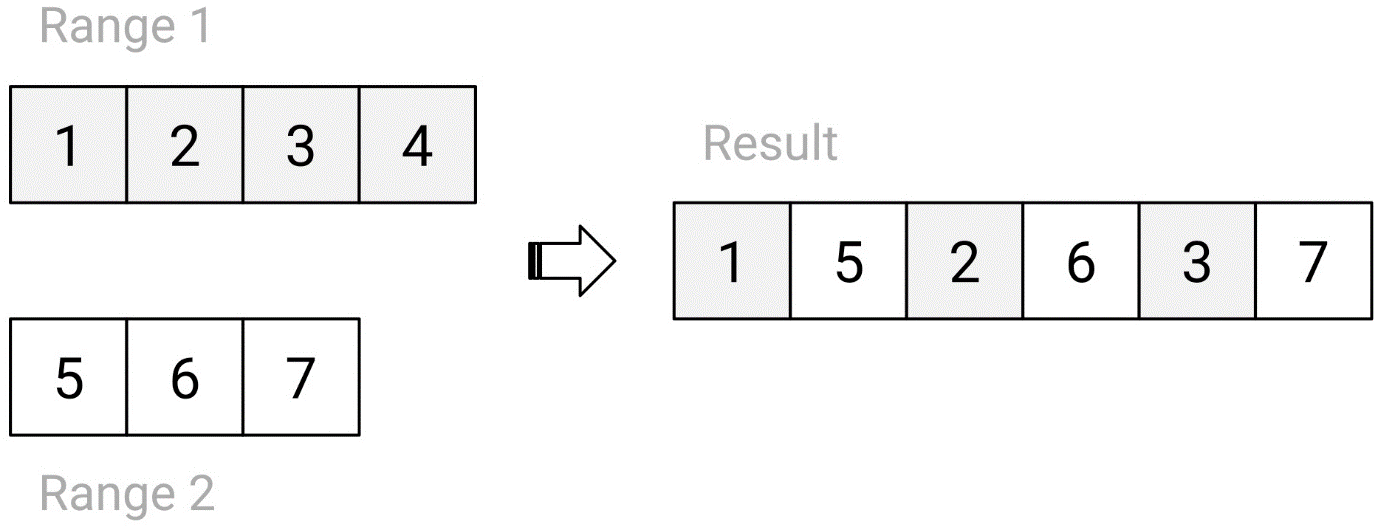
\includegraphics[width=0.6\textwidth]{content/3/chapter8/images/4.png}\\
图 8.4
\end{center}

另一些人认为,zip是获取两个或多个输入范围并创建一个新范围,其中元素是由输入范围的元素组成的元组。如下图所示:

\begin{center}
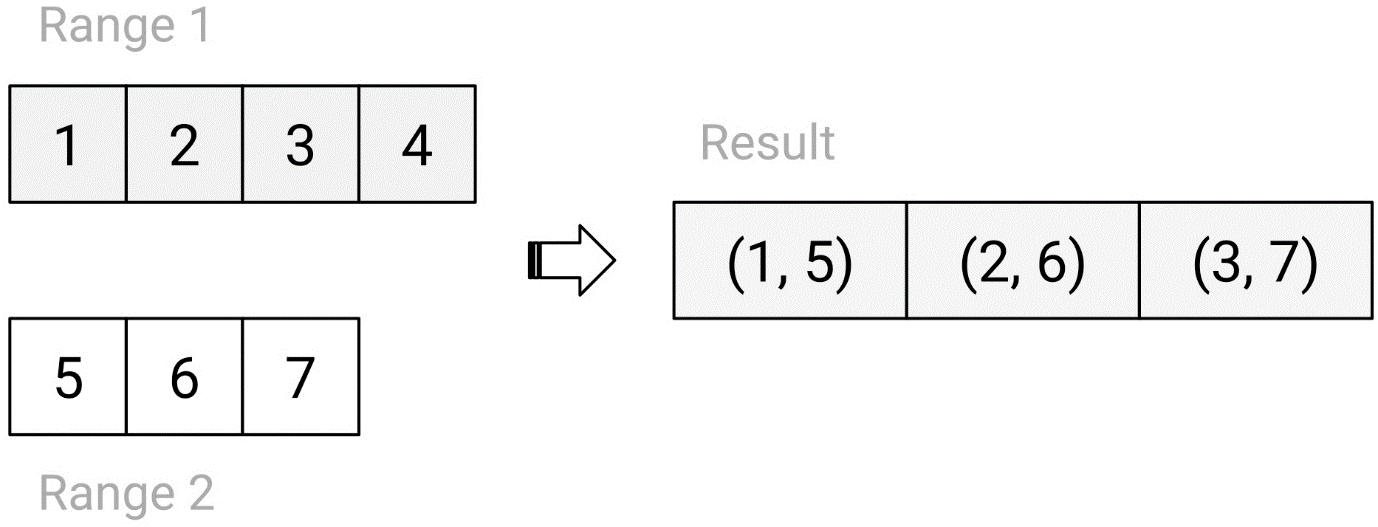
\includegraphics[width=0.6\textwidth]{content/3/chapter8/images/5.png}\\
图 8.5
\end{center}

本节中,我们将实现第一个算法。为了避免混淆,将其称为flatzip。以下是其要求:

\begin{itemize}
\item
该算法接受两个输入范围并写入一个输出范围。

\item
算法以迭代器作为参数。对第一个和最后一个输入迭代器定义了每个输入范围的边界,输出迭代器定义了将写入元素的输出范围的开始位置。

\item
两个输入范围应该包含相同类型的元素。输出范围必须具有相同类型的元素,或者输入类型可隐式转换为的类型。

\item
若两个输入范围的大小不同,当两个输入范围中最小的一个被处理时,算法就会停止(如前图所示)。

\item
返回值是复制倒数第一元素的输出迭代器。
\end{itemize}

所描述的算法的可能实现如下所示:

\begin{lstlisting}[style=styleCXX]
template <typename InputIt1, typename InputIt2,
		  typename OutputIt>
OutputIt flatzip(
	InputIt1 first1, InputIt1 last1,
	InputIt2 first2, InputIt2 last2,
	OutputIt dest)
{
	auto it1 = first1;
	auto it2 = first2;
	
	while (it1 != last1 && it2 != last2)
	{
		*dest++ = *it1++;
		*dest++ = *it2++;
	}

	return dest;
}
\end{lstlisting}

实现非常简单。这里所做的只是同时遍历两个输入范围,并交替地从它们复制元素到目标范围。当到达最小范围的终点时,两个输入范围上的迭代停止。可以这样使用算法:

\begin{lstlisting}[style=styleCXX]
// one range is empty
std::vector<int> v1 {1,2,3};
std::vector<int> v2;
std::vector<int> v3;

flatzip(v1.begin(), v1.end(), v2.begin(), v2.end(),
		std::back_inserter(v3));
assert(v3.empty());

// neither range is empty
std::vector<int> v1 {1, 2, 3};
std::vector<int> v2 {4, 5};
std::vector<int> v3;

flatzip(v1.begin(), v1.end(), v2.begin(), v2.end(),
		std::back_inserter(v3));
assert(v3 == std::vector<int>({ 1, 4, 2, 5 }));
\end{lstlisting}

这些例子对输入和输出范围都使用std::vector,但flatzip算法对容器一无所知。容器的元素可以在迭代器的帮助下访问,所以只要迭代器满足指定的要求,就可以使用任何容器。这包括我们之前编写的circular\_buffer容器,因为circular\_buffer\_container同时满足输入和输出迭代器类别的要求。还可以编写如下代码:

\begin{lstlisting}[style=styleCXX]
circular_buffer<int, 4> a({1, 2, 3, 4});
circular_buffer<int, 3> b({5, 6, 7});
circular_buffer<int, 8> c(0);

flatzip(a.begin(), a.end(), b.begin(), b.end(), c.begin());

std::vector<int> v;
for (auto e : c)
	v.push_back(e);
assert(v == std::vector<int>({ 1, 5, 2, 6, 3, 7, 0, 0 }));
\end{lstlisting}

这里有两个输入循环缓冲区:a有四个元素,b有三个元素。目标循环缓冲区的容量为8个元素,全部初始化为0。应用flatzip算法之后,目标循环缓冲区的六个元素将使用a和b缓冲区中的值写入。结果是循环缓冲区将包含元素1,5,2,6,3,7,0,0。













